\documentclass[aspectratio=169, 10pt]{beamer}

\usepackage{caption}

\hypersetup{
    colorlinks=true,
    linkcolor=blue,
    filecolor=magenta,      
    urlcolor=cyan
}

\usetheme{metropolis}

\logo{
\includegraphics[height=10pt]{cross-logo-wide.png}}

\title{Reproducible Computational Science\\ with Popper Workflows}
\subtitle{CROSS 2020 Research Symposium}
\titlegraphic{
\includegraphics[height=30pt]{cross-logo-wide.png}}
\author{Anders Poirel}
\date{}
\institute{ University of California, Santa Cruz}

\begin{document}

\maketitle

\begin{frame}{Common Reproducibility Issues (1)}
    \begin{columns}
        \begin{column}{0.5\textwidth}  %%<--- here
            \begin{center}
                \begin{figure}
                    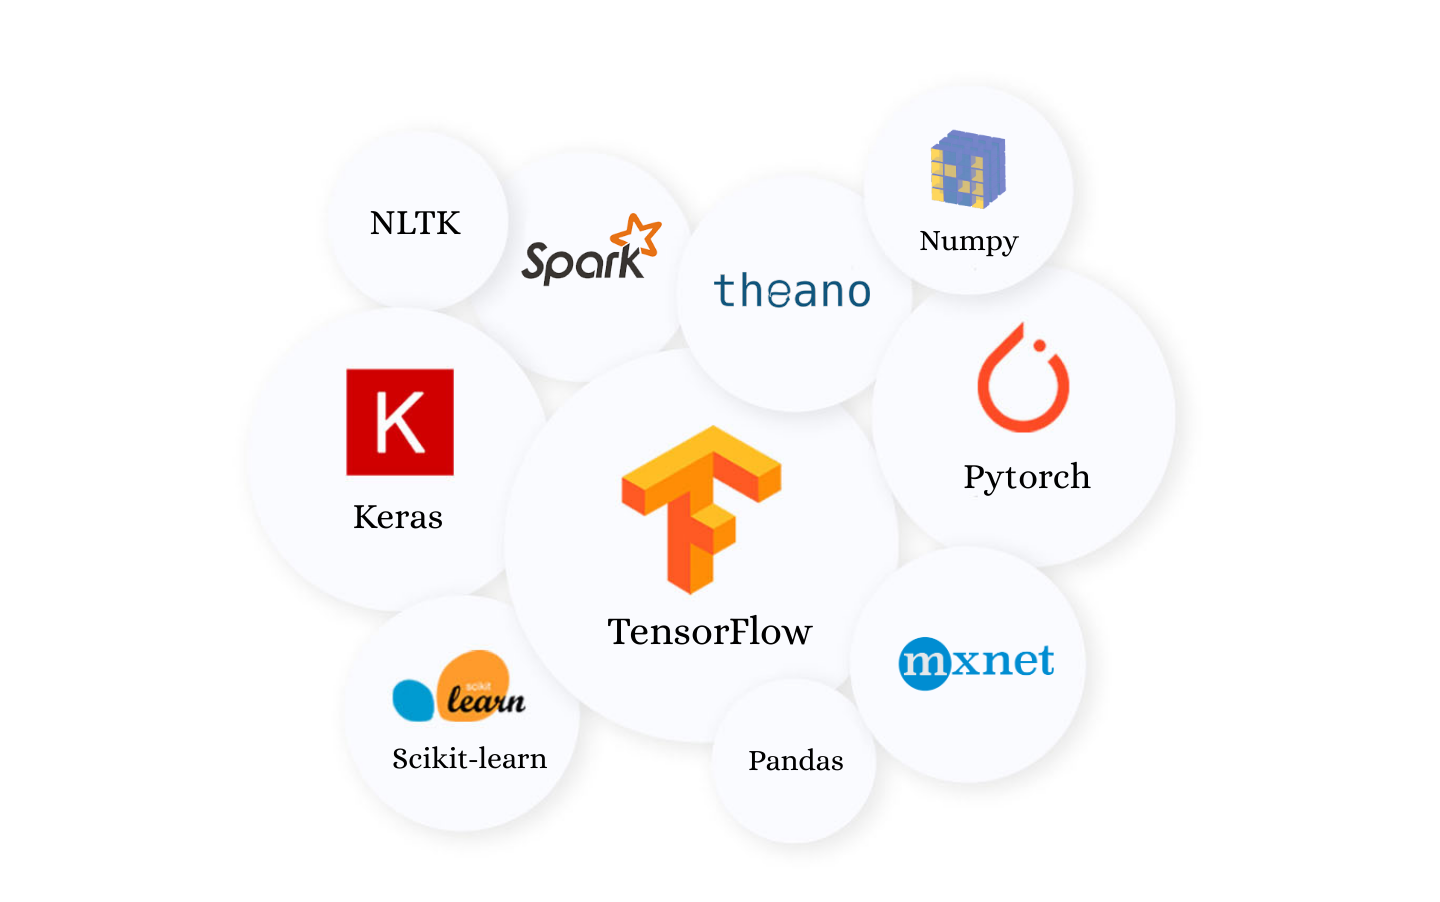
\includegraphics[width=1.1\textwidth]{images/libraries.png}
                    \caption*{{\sl Python statistics libraries}}
                \end{figure}
            \end{center}
        \end{column}
        \begin{column}{0.5\textwidth}
            \begin{itemize}
                \item Research using statistical and/or machine learning tools
                depends on increasingly complex software stacks
                \item Replicating a result is difficult due to 
                incomplete dependencies, platform incompatibilities, $\ldots$ 
            \end{itemize}
        \end{column}
    \end{columns}
\end{frame}

\begin{frame}{Common Reproducibility Issues (2)}
    \begin{columns}
        \begin{column}{0.5\textwidth}  %%<--- here
            \begin{center}
                \begin{figure}
                    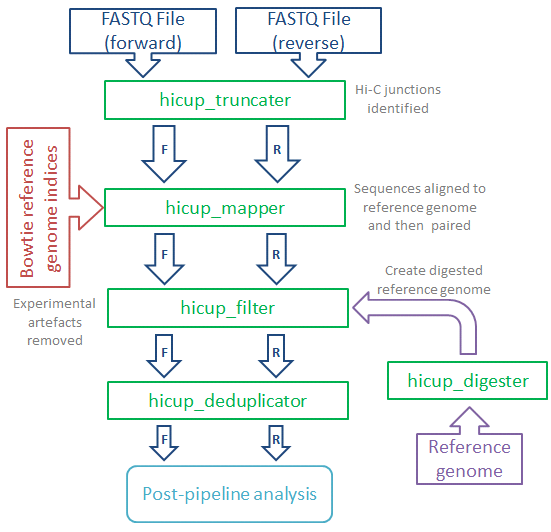
\includegraphics[width=\textwidth]{images/pipeline.png}
                    \caption*{{\sl A bioinformatics data pipeline}}
                \end{figure}
            \end{center}
        \end{column}
        \begin{column}{0.5\textwidth}
            \begin{itemize}
                \item Data processing pipelines have many interdependant steps
                from the raw data to the final result 
                \item Replicating a workflow requires difficult guesswork if these steps not properly documented 
            \end{itemize}
        \end{column}
    \end{columns}
\end{frame}

\begin{frame}{Popper}
    \begin{columns}
        \begin{column}{0.5\textwidth}  %%<--- here
            \begin{center}
                \begin{figure}
                    
\includegraphics[width=0.8\textwidth]{images/popper_logo.png}
                \end{figure}
            \end{center}
        \end{column}
        \begin{column}{0.5\textwidth}
            Popper is a container-native workflow execution engine
            which addresses these issues:
            \begin{itemize}
                \item Containerizing workflows avoids problems due to different 
                software environments
                \item Specifying steps explicitely in a Popper workflow file avoids problems due to data pipeline complexity
            \end{itemize}
        \end{column}
    \end{columns}

\end{frame}

\begin{frame}{Limitations}
    However $\ldots$
    \begin{itemize}
        \item  Popper requires fluency in DevOps tools (in particular
        container engines)
        \item Steep learning curve for users with no prior experience in these tools, who would nonetheless benefit from more reproducible workflows
    \end{itemize}
    $\rightarrow$ My goal was to create a collection of tools and tutorials
    to smooth out this learning curve for users in computational fields 
\end{frame}

\begin{frame}{Contributions: Tutorials}
    Tutorial for developing Popper workflows oriented to Python and R users:
    \begin{itemize}
        \item Computational notebooks with Popper 
        \item Dependency management
        \item Project structure
    \end{itemize}
\end{frame}

\begin{frame}{Contributions: Templates}
    \alert{cookiecutter} templates to bootstrap Popper workflows in Python and R
    including starter Docker images
    \begin{center}
        \begin{figure}
            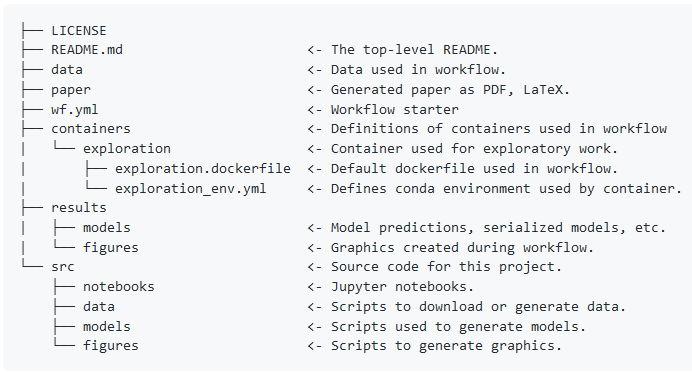
\includegraphics[width=0.6\textwidth]{images/project_structure.png}
            \caption*{{\sl Structure generated by cookiecutter for Python workflows}}
        \end{figure}
    \end{center}
\end{frame}

\begin{frame}{Contributions: Sample Workflows}
    \begin{columns}
        \begin{column}{0.5\textwidth} 
            \begin{center}
                \begin{figure}
                    
\includegraphics[width=0.2\textwidth]{images/workflow.png}
                    \caption*{{\sl Workflow diagram generated by Popper}}
                \end{figure}
            \end{center}
        \end{column}
        \begin{column}{0.5\textwidth}
            Sample Popper workflows in Python and R demonstrating an end-to-end 
            machine learning project with data acquisition and transformation,
            model fitting and evaluation
        \end{column}
    \end{columns}   
\end{frame}

\begin{frame}{Highlights (1)}
    \begin{itemize}
        \item \textbf{Key idea in DevOps}: minimize the distance between development 
        and production environments 
        \item Users in computational research should be able to develop from the beginning their workflows in Popper 
        \item This is done using Popper's interactive execution feature
    \end{itemize}
\end{frame}

\begin{frame}{Highlights (2)}
    \begin{columns}
        \begin{column}{0.5\textwidth} 
            \begin{center}
                \begin{figure}
                    
\includegraphics[width=0.5\textwidth]{images/jupyter.png}
                \end{figure}
            \end{center}
        \end{column}
        \begin{column}{0.5\textwidth}
            \begin{itemize}
                \item Users in computational fields use computational
                notebooks to prototype workflows 
                \item I added configuration options to the core \alert{popper} CLI 
                to support running a computational notebook server
            \end{itemize}
        \end{column}
    \end{columns}  

\end{frame}


\begin{frame}{Thank you!}
    I'd like to thank Ivo Jimenez for his mentorship this summer!
\end{frame}





\end{document}